\chapter{Kurs 3472}
\section{Diversit"at}
\subsection{Fragen und Antworten zum Text von \textcite{stahlberg_geschlechterdiskriminierung_2009}}
\subsubsection{Welche normativen und "okonomischen Probleme ergeben sich aus der Benachteiligung von Frauen?}
Ein normatives Problem ergibt sich, wenn eine Gesellschaft sich Gleichberechtigung auf die Fahne schreibt, die dann aber nicht gegeben ist. Ein "okonomisches Problem ist es, wenn Geld daf"ur ausgegeben wird, Frauen auszubilden, diese Investition aber nicht wieder reingeholt wird, weil Frauen nicht in Jobs kommen.

\subsubsection{Welche Aspekte umfasst der Oberbegriff Geschlechtsstereotyp?}
\begin{itemize}
        \item Pers"onlichkeitseigenschaften
        \item Rollenverhalten
        \item kognitive F"ahigkeiten
        \item physische Merkmale
\end{itemize}

\subsubsection{Wodurch unterscheiden sich deskriptive und pr"askriptive Geschlechtsstereotype?}
\emph{Deskriptiv} ist eine Beschreibung dessen, wie sich M"anner oder Frauen tats"achlich verhalten. \emph{Pr"askriptiv} meint, wie sich verhalten sollen.

\subsubsection{Welche Begriffe beschreiben die in weiblichen und m"annlichen Stereotypen enthaltenen Eigenschaften?}
Weiblich:
\begin{itemize}
        \item Warmherzigkeit
        \item Communion
        \item Expressivit"at
\end{itemize}

\noindent M"annlich:
\begin{itemize}
        \item Kompetenz und Rationalit"at
        \item Agency
        \item Instumentalit"at
\end{itemize}

\subsubsection{Was ist moderner, subtiler oder wohlmeinender Sexismus und weshalb ist er problematisch?}
Sie sind nicht so leicht als Sexismus zu enttarnen, tragen aber zur Aufrechterhaltung von Diskrimierung bei.

\subsubsection{Welche Unterschiede finden sich zwischen den Geschlechtern?}
Keine Unterschiede bei:
\begin{itemize}
        \item Intelligenz
        \item Motiven
        \item mathematische F"ahigkeiten
        \item Anzahl der Studienanf"anger
        \item Anzahl der Studienabsolventen
\end{itemize}

\noindent Unterschiede bei:
\begin{itemize}
        \item verbale F"ahigkeiten: Frauen besser (aber nur wenig)
        \item "altere Generation: Frauen haben geringeres Bildungsniveau
        \item j"ungere Generation: Frauen haben h"oheres Bildungsniveau
        \item Gehalt: Frauen verdienen ca. 15\% weniger
        \item Beruf: Frauen seltener in F"uhrungspositionen
        \item weniger Frauen bei den Professoren
\end{itemize}

\subsubsection{Wie erfolgt geschlechtstypisierende Darstellung in den Medien?}
\begin{itemize}
        \item weniger Frauen in Hauptrollen
        \item Betonung der stereotypischen Rollen (Betonung von Attraktivit"at bei Frauen)
        \item K"orperhaltung
        \item \emph{Generisches Makulinum}
        \item \emph{Linguistic Expectancy Bias}
\end{itemize}
\subsubsection{Was sind \emph{generisches Maskulinum} und \emph{Linguistuc Expectancy Bias} und wie wirken sie sich aus?}
\begin{description}
        \item[Generisches Maskulinum] Wenn immer nur die maskuline Sprachform verwendet wird.
        \item[Linguistic Expectancy Bias] Stereotyp-kongruentes Verhalten wird abstrakter beschrieben als stereotyp-inkongruentes Verhalten. Z.B. wird "uber positive Ergebnisse von M"annern in F"uhrungspositionen eher etwas allgemeines gesagt wie ``Er kann andere mitreissen.'' "Uber Frauen wird dagegen eher etwas gesagt wie ``Ihr gelang es, Mitglieder aus dem Team zum mitmachen zu bewegen.'' Bei negativen Ergebnissen w"are es dagegen genau anders herum.
\end{description}
\subsubsection{Verschiedene Prozesse und Effekte tragen zur Geschlechterdiskriminierung und Verringerung der Erfolgschancen von Frauen bei. Welche sind das und wie wirken sie sich aus?}
\begin{description}
        \item[Stereotype Threat.] In einer Situation, in der ein Stereotyp aktiviert ist, kann der Druck, der durch dieses Stereotyp erzeugt wird, dazu f"uhren, dass Personen der stereotypisierten Gruppen erwarten, sich im Sinne des Stereotyps zu verhalten. Es kann auch dazu f"uhren, dass sie sich tats"achlich so verhalten. 
        \item [Lack-of-Fit.] Wahrgenommene mangelnde Passung zwischen Eigenschaften einer Person und Anforderung des Berufs. Erfolgserwartungen an diese Person im Beruf sind schlechter, je schlechter die Passung. 
        \item [Think-Manager-Think-Male.] Ein Spezialfall des Lack-of-Fit Modells. Der Managerberuf wird als typisch m"annlich angesehen und Frauen wird nicht zugetraut, diesen Beruf erfolgreich auszu"uben. W"ahrend in den $70$-er Jahren noch beide Geschlechter von diesem Ph"anomen betroffen waren, sind es mittlerweile nur noch die M"anner, die den Frauen den Managerberuf nicht zutrauen.
        \item [Glass Ceiling.] Eine unsichtbare und un"uberwindbare Barriere f"ur Frauen, die Karriere machen wollen.
        \item [Glass Escalator.] Eine unsichtbare Hilfe f"ur M"anner, die Karriere machen wollen. 
        \item [Token-Effek.t] Tokens sind Frauen und M"anner in geschlechteruntypischen Berufen. Der Effekt beschreibt das Verhalten der Mehrheit den Tokens gegen"uber. Sie erfahren mehr Aufmerksamkeit und damit evtl. mehr Druck (Stereotype Threat), Unterschiede zwischen Tokens und Mehrheit werden "uber- und Gemeinsamkeiten untersch"atzt und Tokens werden als typische Vertreter ihrer Gruppe angesehen.
        \item [Queen-Bee Syndrom.] Frauen, die in M"annerberufen erfolgreich sind, stimmen Geschlechtsstereotypen zu. 
        \item [Sex-Role Spillover.] Das "Ubertragen von Geschlechtsrollen auf den beruflichen Kontext. Tritt vor allem bei Tokens auf und ist h"aufiger bei Frauen als bei M"annern, weil es weniger M"anner in typischen Frauenberufen gibt. 
        \item [Backlash-Effekt.] Von Frauen und von M"annern wird geschlechtstypisches Verhalten erwartet. Im Beruf wird aber manchmal Verhalten erwartet, dass der Geschlechtsrolle widerspricht. Das kann zum Backlash-Effekt f"uhren. So kann es Frauen, die sich typisch m"annlich verhalten, passieren, dass sich das negativ f"ur sie auswirkt. Ebenso kann das M"annern Passieren, die sich typisch weiblich verhalten.
\end{description}

\subsection{Fragen und Antworten zum Text von \textcite{sue_racial_2007}}
\subsubsection{Wie ist der Begriff der \emph{Mikroaggressionen} definiert?}
Mikroaggressionen sind kurze verbale, nonverbale oder behaviourale Dem"utigungen. Sie k"onnen intentional oder nicht intentional sein, ebenso wie bewusst oder unbewusst.

\subsubsection{Beschreiben sie die drei Formen von Mikroaggressionen!}
\begin{description}
        \item[Microassault] Ein \emph{Mikroangriff} ist ein expliziter Angriff mit der Intention, die Zielperson zu verletzen. Dementsprechend handelt es sich um bewusste Handlungen, z.B. wenn jemand die Stra"senseite wechselt, weil ihm ein Migrant entgegenkommt.
        \item[Microinsult] Eine \emph{Mikrobeleidigung} zeigt sich in fehlender Sensibilit"at und Herablassung gegen"uber Rasse oder ethnischer Identit"at einer Person. Mikrobeleidigungen k"onnen subtil und f"ur den Beleidgenden unbewusst sein. F"ur den Beleidigten sind sie in aller Regel durchaus bewusst, z.B. wenn ein Deutscher mit Migrationshintergrund wiederholt danach gefragt wird, woher er kommt.
        \item[Microinvalidation] Wenn Gef"uhle, Gedanken oder erlebte Realit"at von Migranten heruntergespielt, negiert oder ganz ignoriert werden. Z.B. ``Alle Menschen sind gleich.''
\end{description}

\subsubsection{Welche vier Dilemmata bestehen im Hinblick auf Mikroaggressionen?}
\begin{itemize}
        \item Unterschiede in der Wahrnehmung von ethnischen Realit"aten
        \item Unsichtbarkeit von nicht intendierten Mikroaggressionen
        \item Wahrgenommener minimaler Schaden
        \item Teufelskreis bei der Reaktion auf Mikroaggressionen
\end{itemize}

\subsubsection{Dilemma 1: Welche Unterschiede bestehen zwischen \emph{people of colour and Whites}?}
\emph{Whites} sind der Meinung, dass es Rassismus effektiv nicht mehr oder kaum noch gibt, und dass Migranten genauso wie sie oder evtl. sogar besser behandelt werden. Die erlebte Realit"at von \emph{people of colour} sieht dagegen ganz anders aus.

\subsubsection{Dilemma 2: Welche Rolle spielt \emph{Colour Blindness}?}
\emph{Farbenblindheit} ist eine schwere Form von Mikroinvalidierung. \emph{Whites} verhalten sich faktisch diskriminierend, beteuern aber, dass ihr Handeln nichts mit der Hautfarbe zu tun habe. Tats"achlich ist es m"oglich, dass ihnen ihr diskriminierendes Verhalten nicht bewusst ist.

\subsubsection{Dilemma 3: Wie werden die Auswirkungen von Mikroaggressionen "ublicherweise eingesch"atzt?}
Sie werden als nicht schwerwiegend eingesch"atzt. Oft ist sich der Diskriminierende ja nicht einmal bewusst, dass er diskriminiert hat. Tats"achlich spricht aber vieles daf"ur, dass Mikroaggressionen schlimmeren Schaden anrichten als traditionelle, offene Aggressionen. Und zwar weil f"ur das Opfer die Frage bleibt, ob es sich um eine Beleidigung gehandelt hat, ob er reagieren soll und wenn ja, wie.

\subsubsection{Dilemma 4: Welche Rolle spielen bisherige Erfahrungen in der Beurteilung von Handlungen als Mikroaggressionen?}
Wie die Frage suggeriert eine Gro"se. Bemerkungen, die als Mikroaggressionen interpretiert werden k"onnen, m"ussen nicht unbedingt solche sein. Es kommt auf den Kontext an. F"ur einen Migranten, der immer wieder Mikroaggressionen ausgesetzt ist, wird ein Verhalten aber eher als rassistisch empfunden, wenn er solches oder "ahnliches Verhalten in anderen Situationen auch schon erlebt hat. Das steht im Gegensatz zum Empfinden des Aggressors, der nur sein Verhalten in der fraglichen Situation kennt, sich also des h"aufigen Vorkommens solcher Situationen nicht bewusst ist.

\subsubsection{Inwiefern spielen Mikroaggressionen eine Rolle im Kontext von Beratung und Therapie?}
F"ur die Beziehung zwischen Klient und Therapeut ist gegenseitiges Vertrauen essentiell. Durch Mikroaggressionen wird dieses Vertrauen gest"ort und kann die Beratung oder Therapie torpedieren.

\subsubsection{Welcher Aspekt von Mikroaggressionen ist die gr"o"ste Herausforderung f"ur Angeh"orige der Majorit"at im Gesundheitswesen?}
Das Unsichtbare sichtbar zu machen. Dies kann nur vollf"uhrt werden, wenn Menschen bereit sind offen und ehrlich den Rassendialog zu f"uhren. Wenn Therapeuten Schwierigkeiten haben das Thema anzusprechen, verschlie�en sie Klienten den Weg dazu, Bereiche der Verzerrung, Diskriminierung und Vorurteile zu erforschen.

 %Sue
\subsection{Fragen und Antworten zum Text von \textcite{mayer_altersdiskriminierung_2009}}
\subsubsection{Was ist Ageism nach Robert Butler?}
Der Begriff umfasst drei Facetten:
\begin{itemize}
        \item Vorurteile gg"u. "alteren Menschen, dem Alter und dem Alternsprozess
        \item soziale Diskrimnierungen "alterer Menschen
        \item institutionelle und politische Praktiken, die Stereotype best"atigen und aufrechterhalten
\end{itemize}

\subsubsection{Wie definieren \textcite{mayer_altersdiskriminierung_2009} Altersdiskriminierung? In welchen F"allen sprechen sie nicht von Altersdiskriminierung, obwohl eine Beeintr"achtigung vorliegt?}
Zwei Punkte sind wichtig f"ur das Vorliegen von Altersdiskriminierung. Die Beeintr"achtigung\ldots
\begin{itemize}
        \item legitimer Anspr"uche
        \item allein aufgrund des Alters
\end{itemize}

Wenn die Diskriminerung z.B. aufgrund von alterskorellierten Merkmalen (Gesundheitszustand, fehlende technische Expertise) erfolgt, oder auch keine legitimen Anspr"uche verletzt (Vermeidung von Gespr"achen, Nicht-Aufnahme in ein junges Team), dann ist das zwar unerw"unscht, aber keine Altersdiskrimierung.

\subsubsection{In welchen Lebensbereichen findet Altersdiskriminierung statt?}
\begin{itemize}
        \item Arbeit und Beruf
                \begin{itemize}
                        \item "Altere nehmen seltener an Weiterbildungsma"snahmen teil
                        \item geringere Chance auf Einstellung
                \end{itemize}
        \item Gesundheitswesen
                \begin{itemize}
                        \item Qualitaet der medizinischen Versorgung
                        \item fehlende Wertsch"atzung in der Interaktion mit dem Arzt
                \end{itemize}
        \item Pflege
                \begin{itemize}
                        \item Babysprache
                        \item Fixierung
                \end{itemize}
        \item Medien
                \begin{itemize}
                        \item es werden nur vitale alte Menschen gezeigt
                        \item oder nur "uber Risiken gesprochen
                \end{itemize}
        \item Rechtswesen
                \begin{itemize}
                        \item Glaubw"urdigkeit bei Zeugenaussagen
                \end{itemize}
\end{itemize}

\subsubsection{Welche individuellen Ans"atze zur Erkl"arung von Altersdiskriminierung werden vorgestellt?}
\begin{itemize}
        \item \textbf{Altersstereotype.} Negative und auch positive Einstellungen gg"u. alten Menschen und dem Altern.
        \item \textbf{"Angste vor Altern und Tod.} Nach der \emph{Terror Management Theory} erinnert die Begegnung mit dem Alter an die eigene Zerbrechlichkeit und kann deshalb als bedrohlich empfunden werden.
        \item \textbf{Alterspezifische Motivationen.} Nach der Theorie der sozio-emotionalen selektivit"at suchen j"ungere Menschen ihre Interaktionspartner eher nach einem m"oglichen Informationsgewinn aus. "Altere Menschen suchen eher emptionale Bed"urfnisbefriedigung.
\end{itemize}

\subsubsection{Welche strukturellen Erkl"arungsans"atze werden vorgestellt?}
\begin{itemize}
        \item \textbf{Intergenerationelle Konflikte.} Es geht um Gruppenkonflikte um begrenzte Ressourcen.
        \item \textbf{Strukturelle und institutionelle Rahmenbedingungen.} Durch den demographischen Wandel steht nicht mehr genug Pflegepersonal zu Verf"ugung.
\end{itemize}
\subsubsection{Welche Vor- und Nachteile hat Diskriminierung f"ur die Dskrimierten und f"ur die Diskriminierenden?}
Nachteile f"ur die Diskriminierten:
\begin{itemize}
        \item finanzielle Verluste
        \item gesundheitliche Sch"aden
        \item R"uckzug aus sozialem Leben
        \item Kompletenzverluste im Sinne selbsterf"ullender Prophezeiungen
        \item Folgen der Aktivierung eines negativen Altersstereotyps (Selbstbild, Leistungsf"ahigkeit, Lebenserwartung)
\end{itemize}

\noindent Bew"altigungsprozesse zur Abpufferung:
\begin{itemize}
        \item Menschen kennen die Schattenseiten des "Alterwerdens, sch"atzen aber die Wahrscheinlichkeit gering ein, selbst betroffen sein zu werden
        \item soziale Abw"artsvergleiche
        \item Distanzierung von der eigenen Altersgruppe
\end{itemize}

\noindent Vorteile f"ur die Diskriminierenden:
\begin{itemize}
        \item Stabilisierung und F"orderung des Selbstwergef"uhls
        \item soziale Zugeh"origkeit und positive Eigengruppenidentit"at
        \item Legitimation sozialer Ungleichheit
        \item Schutz vor negativen altersbezogenen Emotionen
\end{itemize}

\noindent Nachteile f"ur die Diskriminierenden:
\begin{itemize}
        \item Verlust der Potentiale der "alterer Menschen
        \item selbstsch"adigendes Verhalten (irgendwann geh"ort jeder zur Gruppe der "alteren Menschen)
        \item volkswirtschaftliche Kosten
\end{itemize}

\subsubsection{Welche Ma"snahmen zum Abbau und zur Pr"avention von Altersdiskriminierung lassen sich ableiten?}
Individuumszentrierte Ma"snahmen:
\begin{itemize}
        \item F"orderung intergenerationaler Kontakte
        \item Wissensvermittlung
        \item Rollenspiele und Alterssimulationen
        \item F"orderung der Perspektiven"ubernahme
        \item Aufbau von Kompetenzen im Umgang mit "alteren Menschen
\end{itemize}

\noindent Strukturelle Ma"snahmen:
\begin{itemize}
        \item Gesetze (Antidiskrimierungsgesetze, Flexibilisierung von Arbeitszeiten)
        \item Verordnungen (Bauvorschriften, "OPNV)
        \item "Offentlichkeitsarbeit f"ur ein differenziertes und realistisches Altersbild
\end{itemize}

\subsection{Fragen und Antworten zum Text von \textcite{steffens_diskriminierung_2009}}
\subsubsection{Wie kann es sich auswirken, wenn Schwule, Lesben und Bisexuelle aus Angst ihre sexuelle Orientierung verbergen?}
\begin{itemize}
        \item niedriges Wohlbefinden
        \item Gesundheitsbeeintr"achtigungen
        \item Aufrechterhaltung von gesellschaftlichen Ressentiments
        \item Vermeidung von sozialen Kontakten
        \item Ver"argen von Sozialkontakten durch reservierte Haltung
\end{itemize}

\subsubsection{Welche Gesetze gab und gibt es, die zur Diskriminierung oder Gleichstellung beitragen? welche Schritte sind noch notwendig f"ur die tats"achliche Gleichstellung?}
Gesetze:
\begin{itemize}
        \item \S 175 StGB (BRD) stellte sexuelle Handlungen zwischen M"annern unter Strafe (1872 -- 1994, BRD) 
        \item \S 151 stellte homosexuelle Handlungen mit Jugendlichen f"ur M"anner und Frauen unter Strafe (1964 -- 1988, DDR)
        \item Gesetz "uber die eingetragene Lebenspartnerschaft (2001)
        \item AGG (2006)
\end{itemize}

\noindent Notwendig f"ur die tats"achliche Gleichstellung:
\begin{itemize}
        \item Einordnung des Lebenspartnerschaftsrechts in das Personenstandsgesetz ("Offnung der Standes"amter)
        \item Gleichstellung verpartnerter Beamten/innen bei Familienzuschlag und Pension
        \item Gleichstellung der Lebenspartner/innen mit Ehegatten im Steuerrecht
        \item Adoptionsrecht
\end{itemize}

\subsubsection{Was sind Beispiele f"ur strukturelle Diskriminierung?}
\begin{itemize}
        \item Versicherungen
                \begin{itemize}
                        \item keine Lebensversicherungen bei gleichgeschlechtlichen Beg"unstigten
                        \item pauschale Verweisung auf erh"ohtes AIDS-Risiko
                        \item keine g"unstigen Partnertarife
                \end{itemize}
        \item Verweigerung von Bedienung im Gast"attenbereich
        \item Wohnungssuche
\end{itemize}

\subsubsection{Wie hoch ist die Pr"avalenz von allt"aglichen Diskriminierungserfahrungen in Deutschland und "Osterreich?}
Deutschland:
\begin{itemize}
        \item Frauen: Beschimpfungen 36\%, Ausgrenzung 28\%, Aufforderungen zu sexuellen Handlungen 16\%, gezwungen zu sexuellen Handlungen 8\%
        \item M"annern: Beschimpfungen 39\%, bedr"angt 14\%, bespuckt 4\%, beworfen 5\%, Eigentum besch"adigt 8\%, bestohlen 9\%, beraubt 4\%, k"orperlicher Angriff (nicht verletzt) 10\%, k"orperlicher Angriff (leicht verletzt) 5\%, k"orperlicher Angriff (schwer verletzt) 1\%
\end{itemize}

\noindent "Osterreich:
\begin{itemize}
        \item Frauen: 13\% verbale Diskriminierung, 13\% k"orperliche Gewalt
        \item M"anner: 21\% verbale Diskriminierung, 24\% k"operliche Gewalt
\end{itemize}

\subsubsection{Warum werden schwule M"anner st"arker diskriminiert als bisexuelle Frauen?}
\begin{itemize}
        \item M"anner "uben eher Gewalt aus, und das auch eher gegen M"anner
        \item Heterosexuelle finden Schwule schlimmer als Lesben
        \item Bisezuelle werden evtl. eher als heterosexuell wahrgenommen, Schwule dagegen sind leichter als solche zu erkennen
\end{itemize}

\subsubsection{Warum werden Konversionstherapien heute nicht mehr empfohlen?}
\begin{itemize}
        \item keine empirischen Befunde f"ur gesundheitsf"ordernde Effekte
        \item negative Effekte wie depressive oder "angstliche Symptome
\end{itemize}

\subsubsection{Was kritisieren \textcite{steffens_diskriminierung_2009} am ICD-10?}
Es gibt immer noch drei Kategorien zur sexuellen Orientierung (die in der Fachwelt als revisionsbed"urftig angesehen werden).

\subsubsection{Worauf sollten Therapeutinnen in der Arbeit mit Schwulen und Lesben achten?}
\begin{itemize}
        \item sexuelle Orientierung ist nicht die Ursache eines Problems
        \item Bedeutung der sexuellen Orientierung nicht untersch"atzen
\end{itemize}

\subsubsection{Diskriminierung im Zusammenhang mit sexueller Orientierung, Angst vor Diskriminierung und negative Einstellungen zur eigenen sexuellen Orientierung wirken sich negativ auf die psychische Gesundheit aus. Welche Befunde st"utzen diese Aussagen?}
\begin{itemize}
        \item Mak, Poon, Pun und Cheung (2007) fanden in einer Metanalyse signifikante Beziehungen zwischen Stigmatisierung und allen 3 Kriterien
        \item Pl"oderl, Trembley und Fartacek (2007) fanden eine erh"ohte Pr"avalenz von Suizidversuchen bei (verbaler oder k"operlicher) Diskriminierung
        \item De Graf, Sandford und ten Have (2006) fanden ein erh"ohtes Suizidrisiko von homosexuellen gg"u. heterosexuellen M"annern in einer niederl"andischen repr"asentativen Stichprobe
        \item Mays und Cochran (2001) fanden erh"ohte Pr"avalenzen f"ur wahrgenommene Diskriminierung und psychische St"orungen in einer amerikanischen repr"asentativen Stichprobe von Schwulen, Lesben und Bisexuellen gg"u. Heterosexuellen
\end{itemize}

%\subsection{Fragen und Antworten zum Text von \textcite{chen_why_2004}}

\subsubsection{Wie verl"auft der Zusammenhang zwischen sozio"okonomischem Status und Gesundheit? }
Positiv: steigender SES -> steigende Gesundheit: \\
Gradient: jede h"ohere Stufe des SES geht mit einem inkrementellen Vorteil f"ur die Gesundheit einher.

\subsubsection{Welche Erkl"arungen f"ur den Zusammenhang zwischen sozio"okonomischem Status und Gesundheit wurden vorgeschlagen? }
Forscher haben viele Erkl"arungen hierzu vorgeschlagen:
\begin{itemize}
        \item genetische Einfl"usse
        \item Umwelteinfl"usse
        \item Giftstoffe
        \item Qualit"at der medizinischen Versorgnung
        \item psychologische und verhaltensbasierte Faktoren
\end{itemize}

\subsubsection{In welche vier Kategorien lassen sich die psychologischen und verhaltensbasierten Erkl"arungsans"atze gruppieren? Nennen Sie Forschungsbefunde f"ur jede der Kategorien. }
\begin{enumerate}
        \item Stress:
                \begin{itemize}
                        \item niedrigerer SES >> mehr negative Ereignisse werden erlebt (Stressoren) >> gr"o"sere negative Auswirkungen wahrgenommen (stress appraisal)
                        \item Stress ist ein plausibler Mediator in der Beziehung zwischen SES und Gesundheit
                        \item Vermutung: wenn der SES einer Person sinkt, nimmt die Menge an erlebtem Stress zu >> wirkt sich wiederum als Tribut auf den K"orper aus
                \end{itemize}
        \item Psychische Belastung:
                \begin{itemize}
                        \item niedrigerer SES >> anf"alliger f"ur das Erleben negativer emotionaler Zust"ande >> biologische Konsequenzen >> ggf. schlechtere Gesundheit
                \end{itemize}
        \item Pers"onlichkeitsfaktoren
                \begin{itemize}
                        \item Personen mit niedrigerem SES besitzen Pers"onlichkeitseigenschaften, die sch"adlich f"ur die Gesundheit sind
                        \item Bspw.: Misstrauen, zynische Haltung, Feindseligkeit, weniger Optimismus >> erh"ohtes Risiko f"ur Krankheiten
                \end{itemize}
        \item Gesundheitsverhalten 
                \begin{itemize}
                        \item niedriger SES >> weniger wahrscheinlich, dass gesunde Verhaltensweisen wie Sport, gesunde Ern"ahrung und Nichtrauchen ausge"ubt werden
                        \item kann an der Verf"ugbarkeit von Ressourcen liegen
                        \item Personen mit eingeschr"anktem Zugang zu gesunden Produkten in ihrer Nachbarschaft werden Schwierigkeiten bei einer gesunden Ern"ahrung haben 
                \end{itemize}
\end{enumerate}

ACHTUNG: Die meisten obigen Faktoren fokussieren auf das Individuum. Beim Versuch die Gesundheit von Kindern zu verstehen, ist es besonders wichtig die Rolle der Familie und der weiteren Umgebung zu betrachten

\subsubsection{Welche drei Modelle versuchen die Entwicklung des Zusammenhangs zwischen sozio"okonomischem Status und Gesundheit in Kindheit und Jugendalter zu beschreiben und wie erkl"aren sie den vorgeschlagenen Verlauf?}
\begin{enumerate}
        \item \textbf{Childhood-limited Model} Beziehung zwischen SES und Gesundheit ist am st"arksten in der fr"uhen Kindheit und wird mit dem Alter schw"acher. Wichtig: Qualit"at der Kinderbetreuung, Bindung an die Eltern, Wohnverh"altnisse
\item \textbf{Adolescent-emergent Model} Beziehungen zwischen SES und Gesundheit sind in der Kindheit schwach und werden mit dem Alter st"arker. Wichtige Faktoren in der Adoleszenz: Peer-Einfluss, bestimmte Pers"onlichkeitsmerkmale
\item \textbf{Persistence Model} Beziehung zwischen SES und Gesundheit ist in Kindheit und Jugendalter "ahnlich 
\end{enumerate}

\subsubsection{Neben der individuellen Ebene k"onnen auch andere Ebenen zur Erkl"arung des Zusammenhangs zwischen sozio"okonomischem Status und Gesundheit herangezogen werden. Welche sind dies und wie k"onnten sie von Bedeutung sein?}
\begin{itemize}
        \item \textbf{Sozialpolitik.} Unterschiedliche Gesellschaften k"onnen verschiedene Ebenen des Vertrauens und des Zusammenhalts zwischen den Communitymitgliedern haben und unterschiedliche Investitionen in die Community f"ordern (Social Capital). Forschung zeigt: Social Capital mediiert den Zusammenhang zwischen SES und Gesundheit.
        \item \textbf{Nachbarschaftsebene.} Hier spielen mehrere Faktoren eine Rolle:
                \begin{itemize}
                        \item gef"ahrliche Nachbarschaften: Barrieren um gesundheitsrelevantes Verhalten auszu"uben
                        \item toxische Umgebungen 
                        \item Grad an Segregation: Segregierte Nachbarschaften investieren tendenziell weniger in "offentliche Dienstleistungen als integrierte Nachbarschaften
                \end{itemize}

        \item \textbf{Familie.} Qualit"ot der Beziehungen innerhalb der Familie. Familien mit vielen Konflikten und kalten, nicht-unterst"utzenden Beziehungen haben eher Kinder, die lebenslang unter gesundheitlichen Problemen leiden und fehlregulierte biologische Systeme aufweisen. 
\end{itemize}

\subsubsection{Welche zwei Bereiche sollten in zuk"unftiger Forschung genauer untersucht werden?}
\begin{enumerate}
        \item st"arker integriertes Verst"andnis des Mechanismus, der hinter der Beziehung von SES und Gesundheit steht durch Ber"ucksichtigung von \emph{gesellschaftlichen}, \emph{Nachbarschafts-}, \emph{Familien-} und \emph{individuellen Variablen}.
        \item dynamische Effekte des SES auf die k"orperliche Gesundheit: welche Art von Auswirkungen auf die Gesundheit sind von welchen Eigenschaften des SES abh"angig?
\end{enumerate}







	
 %gibt's noch nicht
\subsection{Fragen und Antworten zum Text von \textcite{luthar_children_2005}}
\subsubsection{Welche Kohorten wurden untersucht und was waren die Ergebnisse?}

F"ur die Zusammensetzung der Gruppen siehe Tabelle \ref{tab:cohorts}
\begin{table}
        \centering
        \begin{tabular}{c | l | c}
                Name & Klassenstufen & Vergleichsgruppe\\
                \hline
                \hline
                Kohorte 1 & $10$ -- Universit"at & Stadtkinder\\
                Kohorte 2 & $6$ -- $7$ & keine \\
                Kohorte 3 & $6$ -- $11$ & Stadtkinder\\
                \hline
        \end{tabular}
        \caption{Kohorten aus \textcite{luthar_children_2005}.}
        \label{tab:cohorts}
\end{table}

In Kohorte 1 gab es mehr Substanzmissbrauch (Alkohol, Zigaretten, Marihuana) und h"ohere Werte in ""Angstlichkeit und Depression bei wohlhabenden Kindern. Depressionswerte waren f"ur M"adchen h"oher als f"ur Jungen. In den anderen zwei Kohorten wurden die Ergebnisse best"atigt, allerdings treten sie erst ab der $7.$ Klasse auf.

\subsubsection{Leistungsdruck und Isolierung k"onnen bei Kugendlichen mit h"oherem sozio"okonomischen Status zu Problemen f"uhren. Was ist damit gemeint?}
H"ohere Depressionswerte und mehr Substanzmissbrauch f"ur perfektionistische Kinder, Kinder deren Eltern das schulische Abschneiden "uberproportional bewerteten und bei Kindern, die wenig Zeit mit ihren Eltern verbracht haben.

\subsubsection{Die Jugendlichen wurden zu sieben verschiedenen Aspekten des Familienlebens befragt. Welche Unterschiede und Gemeinsamkeiten zwischen den Gruppen zeigten sich?}
Siehe Tabelle \ref{tab:familyaspects}
\begin{table}[hb!]
        \centering
        \begin{tabular}{c | c}
                \hline
                Aspekt & Ergebnis\\
                \hline
                gef"uhlte N"ahe zur Mutter & kein Unterschied\\
                gef"uhlte N"ahe zum Vater & kein Unterschied\\
                Betonung von Integrit"at durch Eltern & kein Unterschied\\
                Regelm"a"siges Abendessen mit Eltern & kein Unterschied\\
                \hline
                Kritik durch Eltern & wohlhabende Kinder besser\\
                Supervision nach der Schule & wohlhabende Kinder besser\\
                \hline
                Erwartungen der Eltern & wohlhabende Kinder schlechter\\
                \hline
        \end{tabular}
        \caption{Ergebnisse der Befragung zu Aspekten des Familienlebens \parencite{luthar_children_2005}.}
        \label{tab:familyaspects}
\end{table}

\subsubsection{Womit h"angt Beliebtheit bei Gleichaltrigen in den Subgruppen zusammen?}
Grunds"atzlich h"angt in beiden Extremgruppen Beliebtheit mit Auflehnung gegen die Obrigkeit zusammen. F"ur genaueres siehe Tabelle \ref{tab:peerstatus}.
\begin{table}
        \centering
        \begin{tabular}{c | c | r}
                \hline
                Gruppe & Geschlecht & Merkmal\\
                \hline
                \hline
                wohlhabende Kinder & M"adchen & geringe schulische Anstrengung\\
                & & Nichtbefolgen von Regeln\\
                & & Aggressivit"at\\
                & Jungen & Substanzmissbrauch\\
                \hline
                Stadtkinder & beide & Aggressivit"at\\
                & & Substanzmissbrauch\\
                \hline
        \end{tabular}
        \caption{Zusammenh"ange von Beliebtheit mit diversen Merkmalen \parencite{luthar_children_2005}.}
        \label{tab:peerstatus}
\end{table}

\subsubsection{Was tr"agt dazu bei, dass Jugendliche aus der Oberschicht oft keine Hilfe bekommen, wenn sie depressiv sind oder andere psychische Probleme haben?}
Schulspychologen und "Arzte tun Probleme von wohlhabenden Kindern oft ab und bewerten sie anders als bei sozial schwachen Kindern. 

\subsubsection{Wie kann es sich auswirken, wenn die psychische Gesundheit von reicheren Jugendlichen vernachl"assigt wird?}
Kinder aus wohlhabenden Familien werden selbst mit hoher Wahrscheinlichkeit zu einflussreichen Pers"onlichkeiten, deren Produktivit"at dann durch eine eventuelle Depression beeintr"achtigt ist. Au"serdem neigen psychisch instabile und ungl"uckliche Personen eher dazu, Ressourcen anzuh"aufen, anstatt sie der Gemeinschaft zur"uckzugeben. (Manche sprechen in diesem Zusammenhang gar von Habgier.)
 %auch wenn es nicht so aussieht: der Text ist an der richtigen Stelle (Luthar)
\subsection{Fragen und Antworten zum Text von \textcite{chen_why_2004}}

\subsubsection{Wie verl"auft der Zusammenhang zwischen sozio"okonomischem Status und Gesundheit? }
Positiv: steigender SES -> steigende Gesundheit: \\
Gradient: jede h"ohere Stufe des SES geht mit einem inkrementellen Vorteil f"ur die Gesundheit einher.

\subsubsection{Welche Erkl"arungen f"ur den Zusammenhang zwischen sozio"okonomischem Status und Gesundheit wurden vorgeschlagen? }
Forscher haben viele Erkl"arungen hierzu vorgeschlagen:
\begin{itemize}
        \item genetische Einfl"usse
        \item Umwelteinfl"usse
        \item Giftstoffe
        \item Qualit"at der medizinischen Versorgnung
        \item psychologische und verhaltensbasierte Faktoren
\end{itemize}

\subsubsection{In welche vier Kategorien lassen sich die psychologischen und verhaltensbasierten Erkl"arungsans"atze gruppieren? Nennen Sie Forschungsbefunde f"ur jede der Kategorien. }
\begin{enumerate}
        \item Stress:
                \begin{itemize}
                        \item niedrigerer SES >> mehr negative Ereignisse werden erlebt (Stressoren) >> gr"o"sere negative Auswirkungen wahrgenommen (stress appraisal)
                        \item Stress ist ein plausibler Mediator in der Beziehung zwischen SES und Gesundheit
                        \item Vermutung: wenn der SES einer Person sinkt, nimmt die Menge an erlebtem Stress zu >> wirkt sich wiederum als Tribut auf den K"orper aus
                \end{itemize}
        \item Psychische Belastung:
                \begin{itemize}
                        \item niedrigerer SES >> anf"alliger f"ur das Erleben negativer emotionaler Zust"ande >> biologische Konsequenzen >> ggf. schlechtere Gesundheit
                \end{itemize}
        \item Pers"onlichkeitsfaktoren
                \begin{itemize}
                        \item Personen mit niedrigerem SES besitzen Pers"onlichkeitseigenschaften, die sch"adlich f"ur die Gesundheit sind
                        \item Bspw.: Misstrauen, zynische Haltung, Feindseligkeit, weniger Optimismus >> erh"ohtes Risiko f"ur Krankheiten
                \end{itemize}
        \item Gesundheitsverhalten 
                \begin{itemize}
                        \item niedriger SES >> weniger wahrscheinlich, dass gesunde Verhaltensweisen wie Sport, gesunde Ern"ahrung und Nichtrauchen ausge"ubt werden
                        \item kann an der Verf"ugbarkeit von Ressourcen liegen
                        \item Personen mit eingeschr"anktem Zugang zu gesunden Produkten in ihrer Nachbarschaft werden Schwierigkeiten bei einer gesunden Ern"ahrung haben 
                \end{itemize}
\end{enumerate}

ACHTUNG: Die meisten obigen Faktoren fokussieren auf das Individuum. Beim Versuch die Gesundheit von Kindern zu verstehen, ist es besonders wichtig die Rolle der Familie und der weiteren Umgebung zu betrachten

\subsubsection{Welche drei Modelle versuchen die Entwicklung des Zusammenhangs zwischen sozio"okonomischem Status und Gesundheit in Kindheit und Jugendalter zu beschreiben und wie erkl"aren sie den vorgeschlagenen Verlauf?}
\begin{enumerate}
        \item \textbf{Childhood-limited Model} Beziehung zwischen SES und Gesundheit ist am st"arksten in der fr"uhen Kindheit und wird mit dem Alter schw"acher. Wichtig: Qualit"at der Kinderbetreuung, Bindung an die Eltern, Wohnverh"altnisse
\item \textbf{Adolescent-emergent Model} Beziehungen zwischen SES und Gesundheit sind in der Kindheit schwach und werden mit dem Alter st"arker. Wichtige Faktoren in der Adoleszenz: Peer-Einfluss, bestimmte Pers"onlichkeitsmerkmale
\item \textbf{Persistence Model} Beziehung zwischen SES und Gesundheit ist in Kindheit und Jugendalter "ahnlich 
\end{enumerate}

\subsubsection{Neben der individuellen Ebene k"onnen auch andere Ebenen zur Erkl"arung des Zusammenhangs zwischen sozio"okonomischem Status und Gesundheit herangezogen werden. Welche sind dies und wie k"onnten sie von Bedeutung sein?}
\begin{itemize}
        \item \textbf{Sozialpolitik.} Unterschiedliche Gesellschaften k"onnen verschiedene Ebenen des Vertrauens und des Zusammenhalts zwischen den Communitymitgliedern haben und unterschiedliche Investitionen in die Community f"ordern (Social Capital). Forschung zeigt: Social Capital mediiert den Zusammenhang zwischen SES und Gesundheit.
        \item \textbf{Nachbarschaftsebene.} Hier spielen mehrere Faktoren eine Rolle:
                \begin{itemize}
                        \item gef"ahrliche Nachbarschaften: Barrieren um gesundheitsrelevantes Verhalten auszu"uben
                        \item toxische Umgebungen 
                        \item Grad an Segregation: Segregierte Nachbarschaften investieren tendenziell weniger in "offentliche Dienstleistungen als integrierte Nachbarschaften
                \end{itemize}

        \item \textbf{Familie.} Qualit"ot der Beziehungen innerhalb der Familie. Familien mit vielen Konflikten und kalten, nicht-unterst"utzenden Beziehungen haben eher Kinder, die lebenslang unter gesundheitlichen Problemen leiden und fehlregulierte biologische Systeme aufweisen. 
\end{itemize}

\subsubsection{Welche zwei Bereiche sollten in zuk"unftiger Forschung genauer untersucht werden?}
\begin{enumerate}
        \item st"arker integriertes Verst"andnis des Mechanismus, der hinter der Beziehung von SES und Gesundheit steht durch Ber"ucksichtigung von \emph{gesellschaftlichen}, \emph{Nachbarschafts-}, \emph{Familien-} und \emph{individuellen Variablen}.
        \item dynamische Effekte des SES auf die k"orperliche Gesundheit: welche Art von Auswirkungen auf die Gesundheit sind von welchen Eigenschaften des SES abh"angig?
\end{enumerate}







	
 %Chen
\subsection{Fragen und Antworten zum Text von \textcite{chen_protective_2012}}

\subsubsection{Welche Faktoren auf welchen Ebenen tragen zu gesundheitlichen Ungleichheiten basierend auf  dem sozio"okonomischen Status bei (health disparities)?}
Folgende Faktoren treten auf individueller und Familien- Nachbarschaftsebene auf:
\begin{itemize}
        \item psychosoziale Faktoren:
                \begin{itemize}
                        \item Stress
                        \item negative Emotionen
                        \item schlechte Gesundheitsverhaltensweisen
                \end{itemize}
        \item physikalische Umweltfaktoren: 
                \begin{itemize}
                        \item nachbarschaftliche Umgebungsbebauung
                        \item Umwelteinfl"usse, die die Gesundheit beeintr"achtigen
                \end{itemize} 
\end{itemize}


\subsubsection{Was ist Resilienz und was tr"agt dazu bei auf den Ebenen \emph{des Individuums} \emph{der Familie} und \emph{der Nachbarschaft}? }
Resilienz ist die Anpassung im Angesicht der Bedrohung. Die Literatur identifiziert wichtige Faktoren auf den drei genannten Ebenen. Diese Faktoren wirken als Puffer bei Widrigkeiten und sch"utzen Kinder vor Verhaltensauff"alligkeiten und schulischem Misserfolg.
\begin{itemize}
        \item \textbf{Indivuduum}
                \begin{itemize}
                        \item Temperament
                        \item kognitive Faktoren
                \end{itemize}
        \item \textbf{Familie}
                \begin{itemize}
                        \item elterliche W"arme
                        \item psychische Gesundheit der Eltern
                \end{itemize}
        \item \textbf{Nachbarschaft}
                \begin{itemize}
                        \item positive Schulumgebung
                \end{itemize}
\end{itemize}

\subsubsection{Was ist mit Verlagern (\emph{shifting}) und Beharren (\emph{persisting}) in dem von der Autorin vorgeschlagenen Modell gemeint? }
\emph{Shifting/Verlagern} meint, sich selbst auf die "au�eren Umst"ande einzustellen:
\begin{itemize}
        \item Akzeptanz von Stressoren
        \item positivere Bewertung stressvoller Situationen 
        \item effektive Emotionsregulation in stressvollen Situationen 
\end{itemize}

\emph{Persisting/Beharren} meint, die erfolgreiche Anpassung an dauerhafte Widrigkeiten. Diese Anpassung hilft dabei, in schwierigen Situationen Sinn zu finden und den Optimismus aufrechtzuerhalten:
\begin{itemize}
        \item die Not durch St"arke durchstehen 
        \item Bedeutung finden 
        \item Optimismus, die eigene Zukunft betreffend
\end{itemize}

WICHTIG: Nicht die einzelnen Strategien (shifting oder persisting) wirken sich positiv auf physiologische Reaktionen von Low-SES-Individuen aus, sondern die Kombination beider Strategien.

\subsubsection{Wie k"onnen sich wahrgenommener Sinn des Lebens und Optimismus auf die k"orperliche Gesundheit auswirken?}
Individuen mit niedrigem SES und einem h"oheren Empfinden des Lebens als sinnvoll hatten \emph{niedrigere Konzentration von IL6} (Entz"undungsmarker, der mit Herz-Kreislauferkrankungen in Verbindung gebracht wird). Im Gegensatz dazu war wahrgenommener Sinn des Lebens nicht mit dem IL6-Marker von Individuen mit hohem SES assoziiert.

Individuen mit niedrigem SES und h"oheren Pessimismuswerten (Gegenteil von Optimismus) hatten einen \emph{h"oheren ambulanten Blutdruck} und eine h"ohere Wahrscheinlichkeit f"ur Bluthochdruck als Low-SES Individuen mit niedrigen Pessimismuswerten oder High-SES-Individuen.


\subsubsection{Ist die Kombination der Strategien Verlagern (\emph{shifting}) und Beharren (\emph{persisting}) f"ur Personen mit h"oherem sozio"okonomischen Status ebenso geeignet?}
Nein. Bei High-SES Individuen k"onnen \emph{proaktive Bew"altigungsstrategien}, die auf die Beseitigung von Stressoren gerichtet sind, effektiver sein, da diese im Schnitt mehr Ressourcen besitzen. 

\subsubsection{Chen (2012) beschreibt zwei Studien, in denen sie und ihre Kolleginnen zeigen konnten, wie sich die Kombination von Verlagern (\emph{shifting}) und Beharren (\emph{persisting}) bei niedrigem sozio"okonomischen Status positiv auf die Gesundheit auswirken. Was genau haben sie bei wem gemessen und welche Zusammenh"ange konnten sie finden?}
In einer Stichprobe Erwachsener, wurden die Umst"ande von deren Kindheit beurteilt. Basierend auf 24 Messungen des Risikos "uber sieben physiologische Systeme, wurde ein Index des kumulativen physiologischen Risikos (\emph{allostatic load}) entwickelt. Zur Vorhersage des allostatic load (der Erwachsenen) interagierte der Einsatz von shift-and-persist Strategien (erfasst "uber die Abfrage von Coping-Stilen und Zukunftsorientierung) mit Low-SES-Kindheiten. 

Unter diesen Personen war die Kombination von hohem Verlagern (shifting) und hohem Beharren (persist) mit den niedrigsten allostatic load-Werten assoziiert. Dieser Zusammenhang fand sich nicht bei High-SES-Individuen.\\

Die Effekte von shift-and-persist wurden zudem in einer klinischen Stichprobe mit Kindern, die unter Asthma leiden untersucht. Hier zeigte sich, dass Low-SES-Kinder mit hohen shift-and-persist Werten 
\begin{itemize}
        \item geringere Asthma-Entz"undungswerte aufwiesen 
        \item h"ohere shift-and-persist Werte (sechs Monate sp"ater) 
\end{itemize}
weniger Asthma Beeintr"achtigungen vorhersagen (geringere Schulfehlzeiten, weniger Rettungs-Inhalator Nutzung). Dieser Zusammenhang fand sich nicht bei High-SES-Kindern. Low-SES-Kinder mit hohen shift-and-persist Werten waren 
in ihren klinischen Profilen High-SES-Kindern "ahnlicher, als Low-SES-Kindern mit niedrigen shift-and-persist Werten. 

\subsubsection{Wodurch k"onnen Kinder die Kombination der Strategien Verlagern (\emph{shifting}) und Beharren (\emph{persisting}) lernen? Beschreiben Sie die Studie, mit der Chen und Kolleginnen ihre Hypothesen empirisch untermauern konnten.}
Durch \emph{Vorbilder (role models)} in der fr"uhen Kindheit.\\

Chen und Kollegen f"uhrten Interviews mit gesunden Jugendlichen "uber ihre Vorbilder, wobei sie folgendes bewerteten: 
\begin{itemize}
        \item SES (sozio"okonomischer Status) 
        \item Einsatz von shift-and-persist Strategien 
        \item Indikatoren des Kardiovaskul"aren Risikos (systemische Entz"undungen und Cholesterinwerte) 
\end{itemize}

In dem Ma�e in dem Low-SES-Jugendliche von unterst"utzenden und inspirierenden Vorbildern berichteten, stieg auch deren Einsatz von shift-and-persist Strategien. (High-SES-Individuen zeigten kein solches Muster.) Zudem hing bei Low-SES-Jugendlichen ein h"oherer shift-and-persist Einsatz mit niedrigeren IL6 Werten und niedrigeren Cholesterinwerten zusammen.





























 %Chen
\section{Auswirkung von Diversit"at auf verschiedenen Ebenen}
\reventionsubsection{Fragen und Antworten zum Text von \textcite{van_knippenberg_categorization-elaboration_2010}}
\subsubsection{Wie wirkt sich Diversit"at auf die Leistung einer Arbeitsgruppe aus, wenn man die Perspektive der sozialen Kategorisierung zugrunde legt?}
Negativ.

\subsubsection{Wie wirkt sich Diversit"at auf die Leistung einer Arbeitsgruppe aus, wenn man die Perspektive der informationellen Ressourcen zugrunde legt?}
Positiv.

\subsubsection{Beschreiben sie das \emph{Categorization and Elaboration Model of Work Group Diversity and Group Perforance} Welche Variaben spielen eine Rolle, wenn es darum geht, wie sich Diversit"at auf die Leistung auswirkt und wie stehen diese Variablen miteinander in Zusammenhang?}
Siehe Abbildung \ref{fig:catelab}

\begin{figure}[<+htpb+>]
        \begin{center}
                \begin{tikzpicture}
                        [gross/.style={ellipse, minimum size=1cm,draw},
                        klein/.style={ellipse,font=\small, draw},
                        mod/.style={ellipse,minimum size=1cm,draw=magenta,fill=magenta!20},
                        %modklein/.style={ellipse,font=\small,draw=magenta,fill=magenta!20},
                        med/.style={ellipse,minimum size=1cm,draw=cyan,fill=cyan!20},
                        medklein/.style={ellipse,font=\small,draw=cyan,fill=cyan!20}
                        ]
                        %Diversitaet und Leistung
                        \node [gross] (Diversity) at (0,0) {Diversit"at};
                        \node [gross] (Leistung) at (10,0) {Leistung};
                        \draw [->] (Diversity) -- node(middle)[auto]{} (Leistung);
                        \node [klein,draw=red,thick,fill=red!20] (Demografisch) [above left= 0.6cm and 1cm of Diversity] {Demografisch};
                        \node [klein,draw=green,thick,fill=green!20] (Funktional) [below left= 0.6cm and 1cm of Diversity] {Funktional};
                        \draw [red](Demografisch) -- node[auto]{-}(Diversity);
                        \draw [green](Funktional) -- node[auto]{+}(Diversity);
                        %Elaboration als Mediator
                        \node [med] (Elaboration) [above=of middle] {Elaboration};
                        \draw [->] (Diversity) -- node[auto](divelab){}(Elaboration);
                        \draw [->] (Elaboration) -- (Leistung);
                        %Mediatormodell der demographischen Diversitaet
                        \node [klein,fill=red!20,above=of Demografisch] (Kategorisierung) {Kategorisierung}; 
                        \node [klein,fill=red!20,right=of Kategorisierung] (Bias) {Intergroup Bias};
                        \draw [->] (Demografisch) -- (Kategorisierung);
                        \draw [->] (Kategorisierung) -- (Bias);
                        \draw [->] (Bias) -- (divelab);
                        %Elaborationsprozess
                        \node [medklein] (Diskussion) [above=of Elaboration] {Diskussion};
                        \node [medklein] (Austausch) [left=of Diskussion] {Austausch};
                        \node [medklein] (Integration) [right=of Diskussion] {Integration};
                        \draw [-,cyan] (Diskussion) -- (Elaboration);
                        \draw [-,cyan] (Austausch) -- (Elaboration);
                        \draw [-,cyan] (Integration) -- (Elaboration);
                        %Moderatoren
                        \node [mod] (Ability) [below= 2cm of middle] {F"ahigkeiten};
                        \node [mod] (Motivation) [left=of Ability] {Motivation};
                        \node [mod] (Complexity) [right=of Ability] {Komplexit"at};
                        \draw [->,magenta] (Ability) -- (middle);
                        \draw [->,magenta] (Motivation) -- (middle);
                        \draw [->,magenta] (Complexity) -- (middle);
        \end{tikzpicture}
        \end{center}
        \caption{Das \emph{Categorization and Elaboration Model}. Mediatoren in \textcolor{cyan}{cyan}, Moderatoren in \textcolor{magenta}{magenta}.}
        \label{fig:catelab}
\end{figure}

\subsubsection{Erkl"aren sie die Studie von Kooij-de Bode et al. (2008). Warum wurde die Studie durchgef"uhrt und was zeigte sie?}
Es ging um den vermuteten negativen Effekt der sozialen Kategorisierung in Arbeitsgruppen. Untersucht wurde die Leistung in Gruppen, die entweder divers oder homogen waren. Au"serdem waren die Informationen entweder verteilt oder allen zug"anglich. Die Leistung war am besten in homogenen Gruppen mit verteilten Informationen und am schlechtesten in diversen Gruppen mit verteilten Informationen. Wenn die Informationen allen zug"anglich waren zeigte sich kein Effekt f"ur Diversit"at.

Das zeigt den negativen Effekt, den Intergroup Bias auf die Leistung von Gruppen haben kann.

\subsubsection{Welche M"oglichkeiten gibt es, die Leistung einer Gruppe zu steigern, deren Mitglieder unterschiedlichen Gruppen angeh"oren?}
\begin{itemize}
        \item Wichtigkeit von Elaboration vermitteln
        \item "Uberzeugung, dass Diversit"at gro"sen Wert hat, f"ordern
\end{itemize}

\subsection{Fragen und Antworten zum Text von \textcite{deaux_nation_2006}}
\subsubsection{Welche drei Ebenen beinhaltet Pettigrews (1997) Modell und was ist auf den Ebenen jeweil f"ur Migrantinnen relevant?}
Die drei Ebenen sind \emph{Makro-}, \emph{Meso-} und \emph{Mikroebene} (siehe Fig. \ref{fig:deaux1}).

\begin{figure}[hb!]
        \begin{center}
                \begin{tikzpicture}[every node/.style={ellipse,draw,text centered,minimum size=3cm,text width=6cm}]
                        \node at (0,0) (makro) { {\large \scshape Makro: soziale Strukturen} {\footnotesize Immigrationspolitik, Demographische Muster, soziale Repr"asentationen}};
                        \node [below=of makro] (meso) { {\large \scshape Meso: soziale Interaktion} {\footnotesize Intergruppenkontakt, Stereotype, Netzwerke}};
                        \node [below=of meso] (mikro) { {\large \scshape Mikro: Individuen} {\footnotesize Einstellungen, Werte, Erwartungen, Motivation, Erinnerungen}};
                \end{tikzpicture}
        \end{center}
        \caption{Drei Ebenen nach Pettigrew (1997) aus \textcite{deaux_nation_2006}.}
        \label{fig:deaux1}
\end{figure}

\subsubsection{Was zeigten Esses et al. (2004, 2006) in ihren Studien mit potentiellen Arbeitgebern?}
Migranten werden nicht genauso behandelt wie einheimische B"urger. Bei gleicher Qualifikation werden Migranten schlechter beurteilt. Ein moderierender Faktor f"ur den Zusammenhang sind Einstellungen gegen"uber Immigration.

\subsubsection{Beschreiben Sie den Versuchsaufbau und die Ergebnisse der Studie zu \emph{stereotype threat} \parencite{deaux_nation_2006}. Wie lassen sich die Ergebnisse und deren Bedeutung auf den verschiedenen Stufen von Pettigrews Modell verstehen?}
Karibische Einwanderer der $1.$ und $2.$ Generation wurden in ihrer Testleistung verglichen. Der Test war vermeintlich indikativ (oder \emph{diagnostisch}) f"ur F"ahigkeiten von Afro-Amerikanern oder nicht. Es zeigte sich der vermutete \emph{Interaktionseffekt} von diagnostischem Test und Zeit in den USA: Einwanderer der $2.$ Generation schnitten schlechter ab, wenn der Test vermeintlich diagnostisch war.\\

Eine "ahnliche Studie wurde mit ethnischer Identifikation durchgef"uhrt. Auch hier gab es einen Interaktionseffekt von diagnostischen Test und ethnischer Identifikation. Bei hoher Identifikation und diagnostischem Test waren die Leistungen schlechter.\\

In Bezug auf Pettigrews Modell: Meso- und Mikroebene sind notwendig, um diese Ergebnisse zu erkl"aren. Auf der Mesoebene werden die Einstellungen (der anderen gegen"uber der eigenen Gruppe) wahrgenommen. Auf der Mikroebene werden die Leistungen schlechter.

\subsubsection{Wie kann zwischen Mikro- und Mesoebene differenziert werden, und welche Interaktionen sind m"oglich? Beschreiben Sie die Untersuchungen und Ergebnisse zum Selbstwertgef"uhl bei verschiedenen Migrantengruppen (Crocker et al., 1994; Wiley, Perkins \& Deaux, 2006)!}
Der soziale Kontext spielt eine wichtige Rolle. Einen Hinweis liefert eine Studie zu privater (wie ich meine Gruppe sehe) und "offentlicher Meinung "uber die Eigengruppe (was ich denke, dass andere "uber meine Gruppe sagen). Bei Wei"sen und Asiaten korrelieren private und "offentliche Meinung. Bei Schwarzen nicht.\\

"Ahnliche Ergebisse gibt es f"ur karibische Einwanderer der $1.$ und $2.$ Generation. Bei Einwanderern der $1.$ Generation korrelieren beide Ma"se, bei Einwanderen der $2.$ Generation tendieren sie gegen Null.

\subsubsection{Was ist mit dem Begriff \emph{remooring (Wiederverankerung)} gemeint? Welche Faktoren beeinflussen, wie dieser Prozess verl"auft?}
Es handelt sich um einen Prozess, in dem jemand in einem neuen Umfeld Wege findet, seine (ethnische) Identit"at aufrecht zu erhalten und sein Selbst zu st"arken. Sehr sch"on ausgedr"uckt wird das durch die "Uberschrift im Text: ``Finding One's Place and Creating a New World''.

Der soziale Kontext ist auch hier ein Faktor. Diskriminierung kann z.B. dazu f"uhren, dass keine (oder nur eine schwache) Ann"aherung an die dominante Kultur stattfindet (etwa bei Mexikanern in den USA) und das, obwohl schon lange immigriert.
 %Deaux
\subsection{Fragen und Antworten zum Text von \textcite{aberson_diversity_2010}}
\subsubsection{Wie lautet die Definition von \emph{Diversit"atserfahrungen} nach \textcite{aberson_diversity_2010}? Inwiefern unterscheidet sich diese Definition von \emph{Intergruppenkontakt}? Welche Beziehung besteht zwischen den beiden Variablen?}
\emph{Diversit"atserfahrungen} beinhalten nicht unbedingt auch den Kontakt (Teilnahme an einer Veranstaltung, Diversity-Training), umgekehrt aber schon. Allerdings ist \emph{Intergruppenkontakt} als ein separates Ph"anomen anzusehen.

\subsubsection{In welche der beiden Kategorien f"allt die Teilnahme an einem Workshop "uber den Islam? Ist die Zusammenarbeit mit Mitgliedern der Fremdgruppe in einem Arbeitskontext nach \textcite{aberson_diversity_2010} eine Diversit"atserfahrung?}
Die Teilnahme an einem Workshop ist eine Diversit"atserfahrung, die Zusammenarbeit mit Mitgliedern der Fremdgruppe ist Kontakt.

\subsubsection{Wie ist der Zusammenhang zwischen Intergruppenerfahrungen und Diversit"atseinstellungen? Auf welche weiteren Variablen wirken sich Diversit"atserfahrungen in \emph{large scale studies} aus?}
Je mehr Intergruppenerfahrungen, desto mehr postive Einstellungen. Au"serdem:
\begin{itemize}
        \item mehr b"urgerliches Engagement
        \item mehr Unterst"utzung f"ur Gleichheit
        \item bessere Perspektiven"ubernahme
        \item mehr positive Interaktionen mit Fremdgruppenmitgliedern
\end{itemize}

\subsubsection{Beschreiben sie die Methode des \emph{Intergroup Dialogue}?}
Studenten aus unterschiedlichen Gruppen diskutieren "uber Unterschiede, Gemeinsamkeiten, soziale Ungleichheit und Wege der Zusammenarbeit zum Abbau von Ungleichheit.

\subsubsection{Welche Erkl"arungen werden f"ur den Befund diskutiert, dass \emph{small scale studies} nicht immer positive Auswirkungen zeigten?}
F"ur diesen Befund wird vor allem die geringe Testst"arke aufgrund von zu kleinen Stichproben verantwortlich gemacht.

\subsubsection{Welche Unzul"anglichkeiten hinsichtlich des Designs von Diversity Trainings werden genannt? Welche Evaluationsdesigns w"aren notwendig?}
\begin{itemize}
        \item keine Kontrollgruppe
        \item nur eine Nachher-Messung
        \item zu wenig Theorie-gest"utzte Programme
\end{itemize}

\subsubsection{Welche Variablen beeinflussen die Wahrscheinlichkeit, dass Personen Diversit"atserfahrungen machen?}
\begin{itemize}
        \item Offenheit f"ur Diversit"at
        \item diverser Freundeskreis
        \item Bewusstsein f"ur soziale Ungerechtigkeit
\end{itemize}

\subsubsection{Welche Variablen konnten als Mediatoren f"ur die Beziehung von Diversit"atserfahrungen und Einstellungen identifiziert werden?}
Siehe Abbildung \ref{fig:aberson1}
\begin{figure}[hb!]
        \begin{center}
                \begin{tikzpicture}
                        [latent/.style={ellipse, minimum size=1cm, draw}]
                        \node [latent] (exp) at (0,0) {Diversit"atserfahrung};
                        \node [latent] (att) at (10,0) {Einstellung};
                        \node (middle) at (5,0) {};
                        \node [latent] (emp) at (5,3) {Empathie};
                        \node [latent] (persp) [above=of emp] {Perspektiven"ubernahme};
                        \node [latent, draw=black!50, color=black!50] (anx) [below=of emp] {"Angstlichkeit};
                        \draw [->] (exp) -- (att);
                        \draw [->] (exp) -- (emp);
                        \draw [->] (exp) -- (persp);
                        \draw [->] (exp) -- (anx);
                        \draw [->] (emp) -- (att);
                        \draw [->] (persp) -- (att);
                        \draw [->] (anx) -- (att);
                \end{tikzpicture}
        \end{center}
        \caption{Mediatoren f"ur den Zusammenhang von Diversit"atserfahrungen und Einstellungen \parencite{aberson_diversity_2010}. "Angstlichkeit konnte - im Gegensatz zur Beziehung von \emph{Intergruppenkontakt} und Einstellungen - nicht als Mediator best"atigt werden. }
        \label{fig:aberson1}
\end{figure}
 %auch dieser Text gehoert an diese Stelle (Aberson)
\section{Identit"at}
\subsection{Fragen und Antworten zum Text von \textcite{amiot_facilitating_2010}}
\subsubsection{Skiziieren sie die unterschiedlichen Phasen des \emph{model of social identity development and integration} \parencite{amiot_facilitating_2010}}
\begin{itemize}
        \item \textbf{Antizipatorische Kategorisierung.} Verankerung der eigenen Identit"at im Vergleich zur neuen Gruppe, bevor ein erster Kontakt stattgefunden hat
        \item \textbf{Kategorisierung.} Konfrontation mit der fremden Gruppe und Realisierung der Unterschiede. Unterschiedliche Gruppenzugeh"origkeit wird salient.
        \item \textbf{Kompartmentalisierung.} Schrittweise "Ubernahme der neuen Identit"at. Alte und neue Identit"at werden aber noch nicht vermischt sondern existieren nebeneinander in distinkten ``Kompartments''.
        \item \textbf{Integration.} Konkrete Anstrengungen um die Konflikte zwischen Identit"aten zu "uberwinden und Gemeinsamkeiten zu finden. Erleben von \emph{Konsistenz} und \emph{Koh"arenz} bez"uglich der eigenen Identit"at.
\end{itemize}

\subsubsection{Grenzen sie dieses Modell von \emph{Social Identity Complexity Theory}, bzw. von \emph{Social Identity/Self Categorization Theory} ab!}

Das \emph{Social Identity Complexity Model} \parencite{brewer_social_2010} beschreibt unterschiedliche Grade der Komplexit"at von Identit"at. Es werden vier Arten genannt, auf die multiple Gruppenzugeh"origkeiten zu einer komplexeren Identi"at kombiniert werden k"onnen. Es wird postuliert, dass diese vier Grade der Komplexit"at auf einem Kontinuum von wenig komplex bis sehr komplex liegen. (Siehe Fig. \ref{fig:amiot1})

\begin{figure}[hb!]
        \begin{center}
                \begin{tikzpicture}
                        [ex/.style={rectangle, draw, text width=15em, text centered, rounded corners, font=\footnotesize},
                        konz/.style={rectangle, draw, text centered, rounded corners}]
                        %Namen der unterschiedlichen Auspraegungen von Komplexitaet
                        \node [konz,blue](inters)     at(0,0)                {Intersection};
                        \node [konz,magenta](domin)     [right=of inters]       {Dominance};
                        \node [konz,green](compar)    [right=of domin]        {Compartmentalization};
                        \node [konz,red](merge)     [right= of compar]      {Merger};
                        \draw [->] (-1, -1) -- (11, -1);
                        \node [font=\tiny] at (-2,-1) {wenig komplex};
                        \node [font=\tiny] at (12,-1) {komplex};
                        %Erlaeuterungen zu den Auspraegungen
                        \node [ex,blue,below= 1cm of inters] (intersex)     {Vereiningung/Schnittmenge aller Identit"aten ist konstituierend f"ur die Identit"at.};
                        \node [ex,magenta,below= 2.3cm of domin] (dominex)   {Es gibt eine prim"are Gruppenzugeh"origkeit. Alle anderen werden untergeordnet.};
                        \node [ex,green,below= 3.5cm of compar] (comparex)   {Multiple Gruppenidentit"aten existieren nebeneinander und werden kontextabh"angig vorgeholt.};
                        \node [ex,red,below= 1cm of merge] (mergeex)    {Differenzierung zwischen Identit"aten bei gleichzeitiger Integration in eine "ubergeordnete Identit"at.};
                \end{tikzpicture}
        \end{center}
        \caption{Kontinuum der Komplexit"at von Identit"at nach dem \emph{Social Identity Complexity Model} \parencite{brewer_social_2010}}
        \label{fig:amiot1}
\end{figure}

Die \emph{Selbstkategorisierungstheorie} zielt im Unterschied zum Entwicklungsmodell von \textcite{amiot_facilitating_2010} auf kurzfristige Kategorisierungsprozesse ab.

\subsubsection{Was ist definierend f"ur die vierte Phase der \emph{Integration} und was unterscheidet diese Phase von der \emph{Compartmentalization}?}
Bei der Integration werden alle multiplem Gruppenzugeh"origkeiten zu einer neuen Identit"at integriert. Dadurch entsteht das Gef"uhl von \emph{Konsistenz, Koh"arenz} und \emph{Authentizit"at}.

\subsubsection{Welche sozialen Faktoren erleichten oder behindern die Integration von neuen Identit"aten? Welche Ansatzpunkte ergeben sich daraus?}
Die zwei Faktoren sind:
\begin{itemize}
        \item Bedrohung
        \item Soziale Unterst"utzung
\end{itemize}

\noindent Die Autoren nennen f"unf Interventionsans"atze:
\begin{itemize}
        \item Anerkennung der Existenz von Diskriminierung und Rassismus
        \item Verst"andnis, dass Bedrohung die Wurzel aller Spannung zwischen Gruppen ist
        \item Entwicklung einer Identit"at, die alle multiplen Gruppenzugeh"origkeiten umfasst (Integration)
        \item Sicherstellung von sozialer Unterst"utzung f"ur Immigranten
        \item Sicherstellung, dass unterschiedliche kulturelle Identit"aten gleicherma"sen wertgesch"atzt werden
\end{itemize}


 %Amiot
\subsection{Fragen und Antworten zum Text von \textcite{nguyen_multicultural_2010}}
\subsubsection{Wie definieren die Autorinnen Multikulturalismus und multikulturelle Identit"at?}
\begin{itemize}
        \item \textbf{Multikulturalismus} bezeichnet die Ber"uhrung mit und die Internalisierung von zwei oder mehr Kulturen.
        \item \textbf{Multikulturelle Identit"at} bezeichnet das Vorhandensein einer starken Bindung mit diesen Kulturen.
\end{itemize}

\subsubsection{Worauf bezieht sich der Begriff Bikulturalismus? Was ist mit Bilingualismus gemeint?}
Bikulturalismis ist der Spezialfall von Multikulturalismus mit genau zwei Identit"aten. Bilingual sind solche Personen, die zwei Sprachen flie"send sprechen.

\subsubsection{Welche Ziele werden mit multikulturellen Ideologien angestrebt und wieso?}
Multikulturelle Ideologien bef"urworten die Inklusion und Gleichwertigkeit aller vorhandenen Kulturen einer Gesellschaft. Es wird angenommen, dass die Anerkennung der eigenen Kultur und M"oglichkeiten der multikulturellen Interaktion zentral f"ur die eigene Kultur und das Wohlbefinden sind. 

\subsubsection{Wie unterscheiden sich Mitglieder einer ethnischen Minorit"at von Mitgliedern der Majorit"at in Bezug auf multikulturelle Ideologien?}
\begin{itemize}
        \item Mitglieder der Minorit"at bef"urworten Multikulturalismus eher als Mitglieder der Majorit"at. 
        \item positiver Zusammenhang von Multikulturalismus und Selbstvertrauen bei Minorit"atsmitgliedern
        \item positiver Zusammenhang von ethnischer Identifikation und Multikulturalismus bei Minorit"atsmitgliedern
        \item negativer Zusammenhang von ethnischer Identifikation und Multikulturalismus bei Majorit"atsmitgliedern
\end{itemize}

\subsubsection{Nennen sie Beispiele daf"ur, wie sich die Adaption einer multikulturellen Ideologie politisch und gesellschaftlich manifestieren kann!}
\begin{itemize}
        \item doppelte Staatsb"urgerschaft
        \item politische Unterst"utzung von Medien in anderen Sprachen
        \item Feiertage 
        \item Gemeindezentren
        \item Akzeptanz von traditioneller Kleidung und Verhaltensweisen
\end{itemize}



\subsubsection{Worin unterscheiden sich klassische und moderne Akkulturationstheorien? Welche Positionen werden empirisch gest"utzt?}
Klassische Akkulturationstheorien gehen von einem eindimensionalen Konstrukt aus, w"ahrend moderne Ans"atze zwei Dimensionen annehmen. Empirische Befunde st"utzen die moderne Sichtweise.

\subsubsection{Skizzieren sie das Akkulturationsmodell von Berry (2003)!}
Siehe Fig. \ref{fig:nguyen1}
\begin{figure}[hb!]
        \begin{center}
                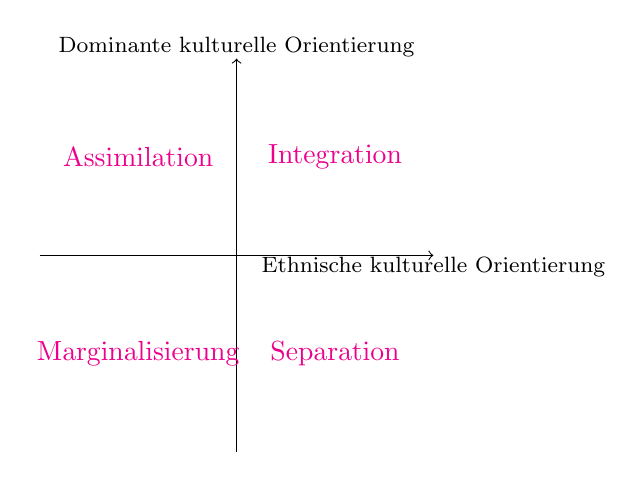
\begin{tikzpicture}
                        [ind/.style={color=magenta},
                        soc/.style={color=cyan},
                        scale=.5]
                        %Koordinatensystem
                        \draw [->] (-5,0) -- (5,0);
                        \draw [->] (0,-5) -- (0,5);
                        \node [font=\footnotesize] at (5,-0.3) {Ethnische kulturelle Orientierung};
                        \node [font=\footnotesize] at (0,5.3) {Dominante kulturelle Orientierung};
                        %Orientierungen
                        \node [ind] (Int) at (+2.5,+2.5) {Integration};
                        \node [ind] (Mar) at (-2.5,-2.5) {Marginalisierung};
                        \node [ind] (Ass) at (-2.5,+2.5) {Assimilation};
                        \node [ind] (Sep) at (+2.5,-2.5) {Separation};
                \end{tikzpicture}
                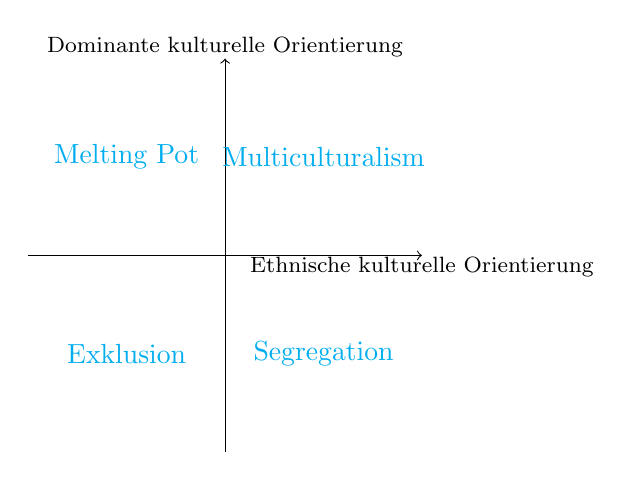
\begin{tikzpicture}
                        [ind/.style={color=magenta},
                        soc/.style={color=cyan},
                        scale=.5]
                        %Koordinatensystem
                        \draw [->] (-5,0) -- (5,0);
                        \draw [->] (0,-5) -- (0,5);
                        \node [font=\footnotesize] at (5,-0.3) {Ethnische kulturelle Orientierung};
                        \node [font=\footnotesize] at (0,5.3) {Dominante kulturelle Orientierung};
                        %Orientierungen
                        \node [soc] at (+2.5,+2.5) {Multiculturalism};
                        \node [soc] at (-2.5,+2.5) {Melting Pot};
                        \node [soc] at (+2.5,-2.5) {Segregation};
                        \node [soc] at (-2.5,-2.5) {Exklusion};
                \end{tikzpicture}
        \end{center}
        \caption{Akkulturationsmodell nach Berry (2003). Links sind die Akkulturationsstrategien auf \textcolor{magenta}{individueller Ebene}, rechts die auch \textcolor{cyan}{gesellschaftlicher Ebene}. Die Achsen gehen (anders als im Studienbrief) von niedrig (links, bzw. unten) nach hoch (rechts, bzw. oben).}
        \label{fig:nguyen1}
\end{figure}

\subsubsection{Was ist mit \emph{cultural frame switching} gemeint?}
Das hin- und herwechseln zwischen kulturellen Orientierungen in Abh"angigkeit der Situation.

\subsubsection{Die Autorinnen schreiben: ``it is important to point out that the acculturation perspective does not presuppose that multicultural individuals internalize and use their different cultures globally and uniformly ''(p. 92). Was ist damit gemeint?}
Verschiedene kulturelle Identit"aten m"ussen nicht in jedem Lebensbereich gleicherma"sen pr"asent sein. Z.B. k"onnte ein Mexikaner in den USA haupts"achlich spanisch sprechen, sich aber trotzdem amerikanischen Werten sehr stark verbunden f"uhlen.

\subsubsection{In welche Typen/Klassen unterteilen (a) LaFromboise et al. (1993), (b) Birman (1994) und (c) Phinney und Devic-Navarro (1997) bikulturelle Personen? Welche Einschr"ankungen/Probleme gehen mit solchen Herausforderungen einher?}
LaFromboise et al. (1993) unterteilen in 2 Klassen: \emph{alternation} und \emph{fusion}.
\begin{itemize}
        \item \textbf{Alternation:} Verhalten passt sich der Situation an (cultural-frame switchers)
        \item \textbf{Fusion:} Orientierung in Richtung einer neuen Kultur
\end{itemize}

\noindent Birman (1994) unterscheidet vier Typen von Individuen:
\begin{itemize}
        \item \textbf{blended:} so wie \emph{fused}
        \item \textbf{instrumental:} Verhalten richtet sich nach beiden Kulturen, Identit"at an keiner von beiden
        \item \textbf{integrated:} Verhalten richtet sich nach beiden, Identit"at nur ethnische Kultur
        \item \textbf{explorers:} Verhalten orientiert sich an dominanter, Identit"at nur an ethnischer Kultur
\end{itemize}

\noindent Phinney und Devich-Navarro (1997) wollen beide Ans"atze integrieren. Sie nehmen zwei Klassen an, die stark an LaFromboise et al. (1993) angelehnt sind:
\begin{itemize}
        \item \textbf{blended biculturals:} Identit"at orientiert sich an beiden Kulturen, kein wahrgenommener Konflikt
        \item \textbf{alternating biculturals:} Identit"at orientiert sich an beiden Kulturen, aber wahrgenommener Konflikt
\end{itemize}

Ein Problem dieser Ans"atze ist  die Vermischung von Verhaltensorientierten und Identit"atorientierten Aspekten. Phinney und Devich-Navarros (1997) Ansatz zielt auf die Identit"at ab, w"ahrend Birmans (1994) Ansatz auf das Verhalten abzielt. LaFromboise et al. (1993( vermischen beides. 

\subsubsection{Wie sollten (bzw. sollten nicht) Akkulturationseinstellungen, Multikulturalismus und Bikulturalismus operationalisert werden? Bergr"unden Sie Ihre Antwort}

Was man machen sollte:
\begin{itemize}
        \item \emph{zweidimensionale Operationalisierung} der kulturellen Orientierungen
        \item \emph{Typologie} mittels Clusteranalyse oder Latent Trait Analyse
        \item \emph{direkte Messung} der Akkulturationsstrategien (mit Einschr"ankungen wg. psychometrischer Probleme)
\end{itemize}

\noindent Was man nicht machen solte:
\begin{itemize}
        \item \emph{eindimensionale Messung.} Hier wird Identifizierung mit einer Kultur gleichgesetzt mit der Nicht-Identifizierung der anderen Kultur.
        \item \emph{Addieren, Subtrahieren oder Multiplizieren} von verschiedenen Orientierungsskalen. Von Vpn mit mittleren Werten wei"s man dann nicht, ob sie auf allen Skalen mittlere Werte angegeben haben, oder auf einer Skala einen hohen  und auf einer anderen einen niedrigen Wert.
        \item \emph{Demographische Variablen zur Akkulturationsmessung.} Akkulturation kann in unterschiedlichen Bereichen in unterschiedlichem Ma"s auftreten. Demographische Variablen eignen sich nicht daf"ur, dass zu erfassen 
\end{itemize}

\subsubsection{Worauf bezieht sich \emph{Bicultural Identity Integration} (BII)? Mit welchen psychologischen Korrelaten h"angt BII zusammen? Aus welchen Komponenten setzt sich BII zusammen?}
BII bezieht sich auf das Ausma"s, in dem Personen ihre beiden kulturellen Identit"aten als gut vereinbar oder als in Konflikt stehend betrachten. Egal, ob hohe oder niegrige Werte f"ur BII erreicht werden, die Identit"at orientiert sich an beiden Kulturen. Vgl. dazu auch Abbildung \ref{fig:bii}.

\begin{figure}[<+htpb+>]
        \begin{center}
                \begin{tikzpicture}
                        [predict/.style={ellipse, draw, text centered, text width=3cm, node distance=3cm},
                        main/.style={ellipse, draw, text centered, thick},
                        correl/.style={ellipse, draw, text centered, text width=3cm,},
                        manifest/.style={rectangle, draw, text centered, rounded corners, font=\footnotesize, node distance=0.2cm}]
                        %Praediktoren und BII
                        \node [main](bii) at (+9,+0) {BII};
                        \node [predict] (dis) [above left=of bii] {Kulturelle Distanz {\footnotesize Kompartmentalisierung vs. "Uberlappung}};
                        \node [predict] (con) [below left= of bii]{Kultureller Konflikt {\footnotesize Spannung vs. Harmonie}};
                        \draw [->] (dis) -- (bii);
                        \draw [->] (con) -- (bii);
                        %Korrelate
                        \node [correl][above left=1cm of dis] (korr11) {Probleme in sozialen Interaktionen};
                        \node [correl][below left=1cm of dis] (korr12) {kontextuelle Herausforderungen};
                        \node [correl][above left=of con] (korr21) {Intrapersonelle Belastungen};
                        \node [correl][below left=of con] (korr22) {Interpersonelle Belastungen};
                        \draw [->] (korr11) -- (dis);
                        \draw [->] (korr12) -- (dis);
                        \draw [->] (korr21) -- (con);
                        \draw [->] (korr22) -- (con);
                        %Manifestationen der Korrelate
                        \node [manifest, above left=of korr11] {Wahrnehmung des eigenen Akzents};
                        \node [manifest, left=of korr11] {Close Mindedness};
                        \node [manifest, left=of korr12] (man1) {kulturell nicht diverse Lebensumgebung};
                        \node [manifest, above =of man1] {sprachliche Schwierigkeiten};
                        \node [manifest, above left=of korr21] {Neurotische Disposition};
                        \node [manifest, below left=of korr21] {wahrgenommene Diskriminierung};
                        \node [manifest, left=of korr22] {Belastungen in interkulturellen Beziehungen};
                \end{tikzpicture}
        \end{center}
        \caption{Zusammenh"ange und Wirkungswege von BII. Kultureller Konflikt und Kulturelle Distanz f"uhren zu BII, es handelt sich also um ein formatives Modell. Praediktoren von Kulturellen Konflikt und Kultureller Distanz sind ebenfalls zu sehen.}
        \label{fig:bii}
\end{figure}

\subsubsection{Welche pers"onlichkeits-, leistungs-, und kontextbezogene Antezedenzien h"angen mit cultural distance und cultural conflict zusammen?}
Vgl. dazu Abbildung \ref{fig:bii}.

\subsubsection{Anhand welcher Kriterien können multikulturelle Personen in f"unf Gruppen eingeteilt werden? Um welche f"unf Gruppen handelt es sich? Wie h"angt BII mit diesen Kriterien und den f"unf Gruppen zusammen?}
Basierend auf \emph{Freiwillligkeit, Mobilit"at} und \emph{Dauer} k"onnen die folgenden f"unf Gruppen unterschieden werden:
\begin{itemize}
        \item Immigranten
        \item Fl"uchtlinge
        \item Sojourners
        \item Ethnische Minorit"aten
        \item Eingeborene
\end{itemize}

Zum Zusammenhang mit BII: Immigranten und Sojourners kommen freiwillig und k"onnen auch wieder gehen. Sie sollten sich also eher auf M"oglichkeiten im Gastland fokussieren, weniger auf Konflikte. Bei Fl"uchtlingen und Eingeborenen ist der Kontakt mit der dominanten Kultur oft erzwungen. Konflikte sollten hier zum Tragen kommen. Bei ethnischen Minorit"aten ist es schwieriger zu sagen. Die erste Generation k"onnte eher den Konflikt zwischen den Kulturen wahrnehmen, w"ahrend nachfolgende Generationen eher keinen Konflikt sehen.

\subsubsection{Welche Effekte kann Multikulturalismus für Individuen und Gesellschaften haben? Welche Variablen moderieren diese Effekte? Welche Ansatzpunkte f"ur die community-psychologische Praxis ergeben sich daraus?}
Auf individueller Ebene kann Multikulturalismus zu besserer \emph{psychologischer und soziokultureller Anpassung} f"uhren. Es besteht au"serdem ein Zusammenhang mit \emph{akademischem Erfolg}, der wiederum der ganzen Gesellschaft dient. Moderiert wird der Zusammenhang von eher kontextuellen Variablen. Wer niemals akzeptiert wird, kann auch schlecht eine integrierte Identit"at entwickeln. Auf der anderen Seite geht das auch nciht, wenn man nie mit ethnischen Minderheiten in Kontakt kommt.





 %Nguyen
\subsection{Fragen und Antworten zum Text von \textcite{simon_when_2013}}
\subsubsection{Auf welche Formen der Mobilisierung bezieht sich die bisherige Forschung zum Zusammenhang von dualer Identifikation und politischer Mobilisierung von Migranten? Wie sieht der Zusammenhang aus?}
Bisherige Forschung konzentriert sich auf legitime politische Mobilisierung, die auch von Mitgliedern der aufnehmenden Gesellschaft akzpetiert wird. Migranten werden so mobilisiert, wenn beide Identit"aten gut zusammen passen.

\subsubsection{Welche m"oglichen Risiken sind mit einer \emph{dual identity} verbunden? Wie k"onnen sie sich auswirken}
Die zwei Identit"aten einer dualen Identit"at k"onnen inkompatibel sein. Das kann zu \emph{Anomie} f"uhren und zu einer politischen Radikalisierung.

\subsubsection{Was ist den zentrale Hypothese? Welches Design wurde gew"ahlt? Was war die zentrale abh"angige Variable und mit welcher Begr"undung wurde sie gew"ahlt?}
Siehe Tab. \ref{tab:simon}.
\begin{table}[h!]
        \centering
        \begin{tabular}{r p{10cm}}
                \hline
                Hypothese & Bei dualer Identit"at f"uhrt wahrgenommene Inkompatibilit"at der Identit"aten zu politischer Radikalisierung.\\
                Design & Paneluntersuchung mit zwei Messzeitpunkten\\
                abh"angige Variable & Sympathie mit radikalen politischen Aktionen\\
                Begr"undung & tats"achlicher politischer Radikalismus ist selten und seine Beobachtung dauert zu lange\\
                \hline
        \end{tabular}
        \caption{Details zur Untersuchung.}
        \label{tab:simon}
\end{table}

\subsubsection{Was ist das zentrale Ergebnis? Benennen sie den Pr"adiktor, den Moderator und die abh"angige Variable!}
Hypothese wurde best"atigt. Bei \emph{hoher wahrgenommener Inkompatibilit"at} (Moderator) besteht ein positiver Zusammenhang zwischen \emph{dualer Identit"at} und \emph{Sympathie f"ur politischen Radikalismus}. (Siehe auch fig. \ref{fig:simon1}.)

\begin{figure}[h!]
        \begin{center}
                \begin{tikzpicture}
                        [konzept/.style={text width=3cm, text centered, minimum height=1.5cm, shape=ellipse, draw}]
                        \node [konzept] at (-5,0) (dual) {Duale Identit"at};
                        \node [konzept] at (+5,0) (symp) {Sympathie f"ur Radikalismus};
                        \node [konzept] at (0,+2) (inko) {Identit"atsinkompatibilit"at};
                        \draw [->] (dual) -- (symp);
                        \draw [->] (inko) -- (0,0);
                \end{tikzpicture}
        \end{center}
        \caption{Moderierte Regression von Identit"atsinkompatibilit"at auf Duale Identit"at.}
        \label{fig:simon1}
\end{figure}

\subsubsection{Beschreiben Sie die Abbildung der Simple-Slope-Analysis (Fig.1, p.5)}
Die Abbildung zeigt die Regressionsgeraden der Regression von politischem Radikalismus auf duale Identit"at in Abhn"angigkeit von wahrgenommener Inkompatibilit"at. Bei hoher Inkompatibilit"at ist die Steigung positiv, bei niedrigerer Inkompatibilit"at dagegen leicht negativ.

\subsubsection{Welches Fazit wird hinsichtlich der kausalen Richtung der Beziehung zwischen dualer Identifikation und Sympathie f"ur Radikalismus bei Personen mit hoher Identit"atsinkompatibilit"at gezogen? Welche Analysen st"utzen diese Schlussfolgerung?}
Die Beziehung soll eben genau so rum sein, wie in der Hypothese formuliert: duale Identit"at bei hoher Identit"atsinkompatibilit"at f"uhrt zu Radikalismus. Um das zu untermauern wurden die gleichen Regressionsanalysen nochmal mit anderen Kriterien durchgef"uhrt:
\begin{itemize}
        \item \textbf{Duale Identifikation (t2).} Sympathie f"ur Radikalismus (t1) hatte einen negativen Effekt.
        \item \textbf{wahrgenommene Inkompatibilit"at (t2).} Sympathie f"ur Radikalismus (t1) hatte einen positiven Effekt.
        \item \textbf{Deren Produktterm.} Sympathie f"ur Radikalismus (t1) hatte keinen Effekt.
        \item \textbf{Bei denen mit hoher Identit"atsinkompatibilit"at:} Kein Effekt von Sympathie f"ur Radikalismus (t1) auf duale Identifikation (t2).
\end{itemize}

\noindent Nochmal auf deutsch: Sympathie f"ur politischen Radikalismus (t2) \emph{steigt} mit dualer Identifikation (t1) (bei Identit"atsinkompatibilit"at), aber duale Identifikation (t2) \emph{sinkt} mit Sympahtie f"ur politischen Radikalismus (t1). 

\subsubsection{Welche Rolle spielt die religi"ose Identit"at?}
Keine Rolle.

\subsubsection{Die Autorinnen schlagen vor, Identit"atsinkompatibilit"at im Rahmen von Mehrebenen-Analysen zu untersuchen. Was bedeutet dieser Vorschlag? Wie k"onnten die unterschiedlichen Ebenen zusammenh"angen? Wie k"onnte eine solche Untersuchung aussehen?}

Der soziale Kontext k"onnte durchaus eine Rolle bei der individuellen Erfahrung von Identit"atsinkompatibilit"at spielen. Es k"onnte z.B. der Fall sein, dass in bestimmten Gegenden Deutschlands die durchschnittliche Inkompatibilit"at h"oher ist als in anderen. 
 %Simon
\subsection{Fragen und Antworten zum Text von \textcite{shih_costs_2010}}
\subsubsection{Was ist \emph{identity switching}? Inwieweit ist dieser Prozess hilfreich, um mit gruppenbezogener Stigmatisierung umzugehen?}
\emph{Identity switching} meint das Betonen von unterschiedlichen Identit"aten in Abh"angigkeit vom Kontext. In einer Situation, in der das Selbstwertgef"uhl durch eine bestimmte Identit"at bedroht ist, kann durch Wechsel der Identit"at der Selbstwert aufrecht erhalten werden.

\subsubsection{Welche f"orderlichen Konsequenzen k"onnen mit einer multiplen sozialen Identit"at (einem komplexen Selbstkonzept) einhergehen?}
Ein komplexeres Selbstbild\ldots
\begin{itemize}
        \item ist ein Puffer gegen Stress und Depression
        \item f"uhrt zu mehr psychischer Gesundheit (z.B. Selbstwirksamkeit, Selbstwertgef"uhl, Zufriedenheit)
        \item erm"oglicht multiple Quellen der sozialen Unterst"utzung
        \item und hat noch ein paar mehr Konsequenzen, die "ahnlich sind
\end{itemize}

\subsubsection{Worauf bezieht sich \emph{identity adaptiveness}? Erkl"aren Sie anhand eines Beispiels aus dem deutschen Kontext!}
\emph{Identity adaptiveness} meint das Ausma"s, in dem eine Identit"at in einem bestimmten Kontext mit einem positiven Stereotyp verbunden ist.

\subsubsection{Wie kann \emph{identity switching} von \emph{frame switching} abgegrenzt werden?}
\emph{(Cultural) frame switching} bezieht sich auf Ph"anomene und Probleme des interkulturellen Austauschs, w"ahrend \emph{identity switching} sich auch Ver"anderungen intraindividueller Art bezieht. Frame switching ist also eher behavioural, identity switching eher perzpetuell.

\subsubsection{Welche Ziele und Vorteile k"onnen durch \emph{identity switching} erreicht werden? Welche Kosten und Nachteile sind damit verbunden?}

\begin{itemize}
        \item \textbf{Vorteile und Ziele}
                \begin{itemize}
                        \item \emph{Passing:} die adaptivere Identit'at in den Vordergrund bringen um seine Ziele zu erreichen
                        \item Selbstwert aufrechterhalten
                        \item Verhindern von negativen Konsequenzen, die mit einer Identit"at verbunden sind
                \end{itemize}
        \item \textbf{Nachteile und Kosten}
                \begin{itemize}
                        \item Fragmentarisierung des Selbst
                        \item Gesundheitliche Folgen bei chronischer Instabilit"at
                \end{itemize}
\end{itemize}

\subsubsection{Welche Faktoren moderieren die Effekte von \emph{identity switching}?}
\begin{itemize}
        \item Inter-domain vs. Intra-domain switching
        \item Anzahl der Identit"aten
        \item Integration der Identit"aten
\end{itemize}

\subsubsection{Erl"autern Sie anhand von konkreten Beispielen, mit welchen Ma"snahmen auf Meso- und Makroebene \emph{identity adaptiveness} gef"ordert werden kann!}
\begin{itemize}
        \item \textbf{Anzahl der verf"ugbaren Identit"aten erh"ohen} z.B. durch m"ogliche Kategorien im Census-Fragebogen
        \item \textbf{Destigmatisierung von Identit"aten} auf Basis von empirischen Befunden (z.B. zu vermeintlichen Geschlechterunterschieden) oder durch Rollenmodelle 
        \item \textbf{Neutrales ``Framing'' von Aufgaben und Kontexten} durch Vermeidung der Betonung von z.B. vermeintlich typisch weiblichen/m"annlichen Attributen (``dies ist ein visuell-r"aumlicher Test'')
\end{itemize}
 %Shih
